\section{Models for Discrete Dependent Variables}
%%%%%%%%%%%%%%%%%%%%%%%%%%%%%%%%
In transportation, there are many cases where the dependent variable of interest is \emph{not continuous}.

Examples:
\begin{enumerate}
	\item Binary: $\begin{cases}
			1 \text{ if you travel to a national park this weekend}\\
			0 \text{ otherwise}
		\end{cases}$
	\item Categorical: mode choice to LAX $\begin{cases}
			\text{ rideshare}\\
			\text{ train}\\
			\text{ shuttle}\\
			\text{ car}
		\end{cases}$
	\item Ranked data
	\item Count data
\end{enumerate}
\subsection{Models for binary outcomes}
	Typically, the values are 0 or 1.  The models shown here are non-linear. They explain the probability of observing either 0 or 1 as an outcome.
	\subsubsection{Statistical model}
		Three ways to introduce these models:
		\begin{enumerate}
			\item Latent variable
			\item Random utility
			\item Probability model
		\end{enumerate}
		\myparagraph{Latent variable approach}
			The latent variable approach (with latent in the meaning of \textit{unobserved}) gives us the probability to observe one outcome for the dependent variable $y$.. Let $y$ be a (0,1) binary variable. Let $x_1,x_2,...,x_{k-1}$ be independent variables we consider using to explain $y$. The key idea is to assume there exists a latent continuous variable $y^*$ which is related to the $x$ as follows:
			\begin{align*}
				y^*_i&=x_i \beta + \epsilon_i\\
				y_i&=\begin{cases}
					1\text{ if } y_i^*>0\\
					0\text{ otherwise}
				\end{cases}
			\end{align*}
			$y^*_i$ can be interpreted as the potential that the event of interest will occur. From our model we know
			\begin{align*}
				Pr(y_i=1|x_i)&=Pr(y_i^*>0|x_i)\\
				&=Pr(x_i \beta > 0 | x_i)=Pr(-\epsilon_i<x_i \beta | x_i)
				&=F(x_i \beta) \longrightarrow
			\end{align*}
			with $F(\cdot)$ as a cumulative distribution statement. Depending on the distributional assumption for $\epsilon_i$, we get different models.
			\begin{itemize}
				\item If $\epsilon_i  \overset{i.i.d.}{\sim}N(0,1)$, we obtain the binary probit model
					\begin{equation*}
						Pr(y_i=1|x_i)=\int\limits_{-\infty}^{x_i \beta} \frac{1}{\sqrt{2 \pi}} e^{-\frac{u^2}{2}} du
					\end{equation*}
				\item If $\epsilon_i  \overset{i.i.d.}{\sim}L(0,\frac{\pi^2}{3})$, we obtain the binary logit model
					\begin{equation*}
					Pr(y_i=1|x_i)=\frac{exp(x_i \beta)}{1+exp(x_i \beta)}
					\end{equation*}
					With $L(\cdot)$ as a logistic distribution. This term represents a \emph{proper} probability because it returns values in the interval $(0,1)$.
			\end{itemize}
			\begin{defi}[Odds function]{defi:oddsf}
				The \emph{odds function} is given by:
				\begin{equation*}
					\Omega(x_i)=\frac{Pr(y_i=1|x_i)}{Pr(y_i=0|x_i)}=\frac{Pr(y_i=1|x_i)}{1-Pr(y_i=1|x_i)}\quad \varepsilon(0,+\infty)
				\end{equation*}
				The odds function represents the ratio of the probability of the event happening (outcome 1) over the event not happening (outcome 0).
			\end{defi}
			For the logit model, the odds function becomes:
			\begin{align*}
				\Omega(x_i)&=\frac{\frac{exp(x_i \beta)}{1+exp(x_i \beta)}}{1-\frac{exp(x_i \beta)}{1+exp(x_i \beta)}}\\
				&=exp(x_i \beta)=e^{x_i \beta}\\
				\Rightarrow ln\left(\Omega(x_i)\right)&=x_i \beta		
			\end{align*}
	\subsubsection{Interpretation}\label{sec:binint}
		\myparagraph{Logit model}
			It is easier to interpret because we have an explicit expression for the model probabilities. As an example, consider the case with 3 explanatory variables:
			\begin{align*}
				\Omega(x_1,x_2,x_3)&=exp(x_0+\beta_1 x_1+\beta_2 x_2 + \beta_3 x_3)\\
				\Omega(x_1+1,x_2,x_3)&=exp(x_0+\beta_1 (x_1+1)+\beta_2 x_2 + \beta_3 x_3)\\
				&=exp(x_0+\beta_1 x_1+\beta_2 x_2 + \beta_3 x_3)\cdot exp(\beta_1)\\
				\Rightarrow exp(\beta_1)&=\frac{\Omega(x_1+1,x_2,x_3)}{\Omega(x_1,x_2,x_3)}
			\end{align*}
			So, for a unit change in $x_i$, the odds change by a factor $e^{\beta_i}$ holding all other variables constant. Note that with $p=Pr(y=1,x)$:
			\begin{align*}
				\Omega&=\frac{p}{1-p}\\
				\Rightarrow \Omega(1-p)&=p\\
				\Rightarrow \Omega&=p(1+\Omega)\\
				\Rightarrow p&=\frac{\Omega}{1+\Omega}			
			\end{align*}
			For the logit, another way to present results is to look at the percentage change in odds:
			\begin{equation*}
				\frac{\Omega(x_1+1,x_2,x_3)-\Omega(x_1,x_2,x_3)}{\Omega(x_1,x_2,x_3)}=(e^{\beta_1}-1)
			\end{equation*}
			\begin{exmp}[Probability of a event in a logit model]{exmp:problog}
				With the latent variable approach:
				\begin{align*}
					y_i&=\begin{cases}
						1 \text{ if } y_i^*\equiv x_i \beta + \epsilon_i \geq 0\\
						0 \text{ otherwise}\\
					\end{cases}\\
					\epsilon_i  &\overset{i.i.d.}{\sim}L(0,\frac{\pi^2}{3})\text{ logit model}\\
					\longrightarrow Pr(y_i=1|x_i)&=\frac{e^{x_i \beta}}{1+e^{x_i \beta}}
				\end{align*}
			\end{exmp}
		\myparagraph{More general interpretation}
			Plot predicted provabilities versus explanatory variables as seen in Figure \ref{fig:logit}. Fix the other explanatory variables and only plot the change over one $x_j$ (only works for the case of $x_j$ being continuous). In case $x_j$ is discrete, generate table of probabilities instead.
			\begin{fig}[Logistic model]{fig:logit}{h}
				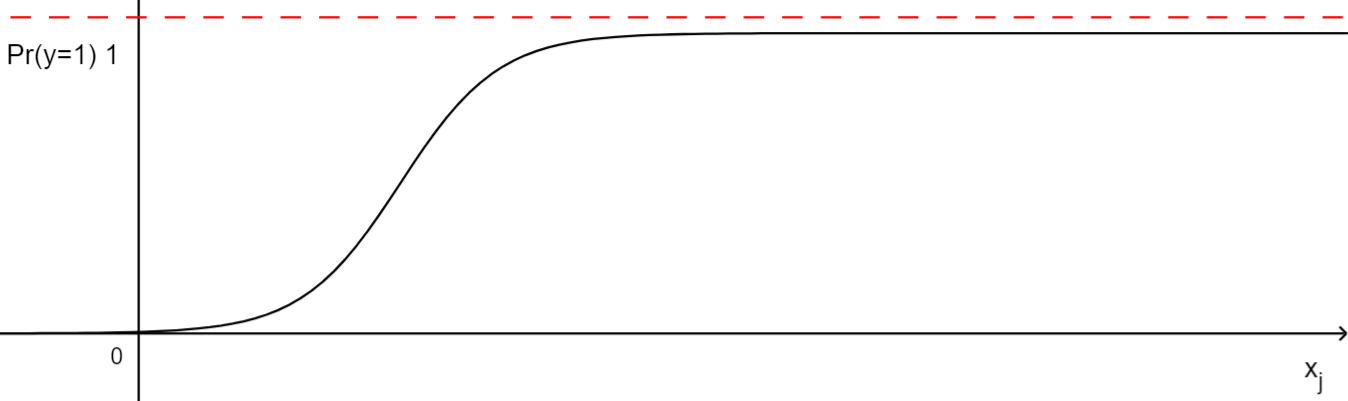
\includegraphics[width=\textwidth]{P18logit.png}	
			\end{fig}				
		\myparagraph{Marginal Changes}
			The third possibility is to report \emph{marginal changes} in probabilities across the sample
			\begin{equation*}
				\frac{\partial Pr(y_i=1|x_i)}{\partial x_{ij}}
			\end{equation*}
			with $x_{ij}$ as a continuous explanatory variable.
	\subsubsection{Measures of fit}\label{sec:mofit}
		A number of different measures of fit have been proposed.
		\begin{itemize}
			\item $Count\,R^2=\frac{\#\,of\,correct\,model\,predictions}{samplesize}$
			\item $McFadden's\,R^2:\,\rho^2=1-\frac{ln(\mathcal{L}^*_{full})}{ln(\mathcal{L}^*_{intercept})}$ where $\mathcal{L}^*_{intercept})$ is the model with no explanatory variables. A larger value indicates a better model.
			\item $McFadden's\,adjusted\,\hat{R}^2:\,\hat{\rho}^2=1-\frac{ln(\mathcal{L}^*_{full})-k}{ln(\mathcal{L}^*_{intercept})}$ with $k$ as the number of $\beta$ in the model (compare to $\bar{R}^2$ for linear regression).
		\end{itemize}
		 The idea of the measures is that if a model is not explaining much, $ln(\mathcal{L}^*_{full})$ is going to be close to $ln(\mathcal{L}^*_{intercept})$ and so McFadden's (adjusted) $R^2$ will be close to 0.
		 		
		 Model parameters are obtained by maximum likelihood. The likelihood function for a random sample is given by
		 \begin{align*}
		 	\mathcal{L}&=\prod_{i=1}^{n} Pr(y_i=1|x_i)^{y_i}\cdot (Pr(y_i=1|x_i))^{1-y_i}\\
		 	y_i&=\begin{cases}
			 	1\\0\\
		 	\end{cases}\\
		 	\text{For the logit: }Pr(y_i=1|x_i)&=\frac{e^{x_i \beta}}{1+e^{x_i \beta}}
		 \end{align*}
		 $\mathcal{L}$ is a product of probabilities $\mathcal{L} < 1$ so $ln(\mathcal{L})< 0$. Hence, $0>ln(\mathcal{L}^*_{full})>ln(\mathcal{L}^*_{intercept})$. In consequence,
		 \begin{equation*}
		 	\frac{ln(\mathcal{L}^*_{full})}{ln(\mathcal{L}^*_{intercept})}\leq 1\text{ so, }1-\frac{ln(\mathcal{L}^*_{full})}{ln(\mathcal{L}^*_{intercept})}\geq 0.
		 \end{equation*}
	\subsubsection{Hosmer-Lemeshow statistic}
		The \emph{Hosmer-Lemeshow statistic} is used to asses if the model is well-specified. The idea is to compare predicted probabilities with observed data. The steps are:
		\begin{enumerate}
			\item Fit the model.
			\item Compute predicted probabilities ($\hat{\pi}_i \equiv Pr(y_i=1|x_i)$).
			\item Sort the data by $\hat{\pi}_i$ from smallest to largest.
			\item Divide observations in $G$ groups ($G\approx 10$), so each group has $\approx \frac{10}{G}$ observations.
			\item Within each group, calculate the mean prediction $\bar{\pi}_g=\left(\sum\limits_{i\varepsilon g} \hat{\pi}_i \right) \frac{1}{n_g}$ with $n_g$ as the number of observations in group $g$.
			\begin{equation*}
				\bar{y}_g=\frac{1}{n_g} \sum\limits_{i\varepsilon g} y_i
			\end{equation*}
			\item Calculate the Hosmer-Lemeshow statistic $HL^*$:
			\begin{equation*}
				HL^*=\sum\limits^{G}_{g=1}\frac{(n_g \bar{y}_g - n_g \bar{\pi}_g)^2}{n_g \bar{\pi}_g (1-\bar{\pi}_g)}
			\end{equation*}
		\end{enumerate}
		If the model is well-specified, $HL^*\sim\chi^2(G-2)$. %todo threshold for decision if it is good or not
	\subsection{Models for nominal outcomes}
		An example for a nominal outcome is mode choice in transportation. This includes unordered variables with more than two outcomes.
		\subsubsection{General model}
			Models are described in more detail in \citetitle{Train.2009} by \textcite{Kennedy.2008}.
			
			Consider a decision maker who has different alternatives for a cause of action. We call this alternatives a \emph{choice set}. We assume that
			\begin{itemize}
				\item these alternatives are mutually exclusive,
				\item the choice set is exhaustive (it contains all alternatives of interest), and
				\item the number of alternatives (elements in the choice set) is finite.
			\end{itemize}
			In addition, it is assumed that the decision maker is going to pick the alternative that maximizes his utility, denoted by $U_{nj}$ where $n$ is an index for the decision maker and $j$ an index for the alternative.
			
			Hence, alternative $i$ is preferred if and only if $\forall\,j\varepsilon\{1,...,J\},\,U_{ni}\geq U_{nj}$ with $J$ number of alternatives.
			
			A researcher does not know the preferences of the decision makers. She observes some of their attributes (stored in vector $s_n$ for decision maker $n$) and some characteristics of each alternative (stored in vector $x_{nj}$). A function is specified that relates $s_n$ ad $x_{nj}$ to decision maker's $n$ utility:
			\begin{equation*}
				V_{nj}\equiv V(x_{nj},s_n)\text{ for }j\varepsilon\{1,...,J\},\,n\varepsilon\{1,...,N\}
			\end{equation*}
			The representative utility $V_{nj}$ is not equal to the actual utility $U_{nj}$ because of incomplete information, expressed by an error term:
			\begin{equation*}
				U_{nj}=V_{nj}+\epsilon_{nj}
			\end{equation*}
			Then, we can express the probability that person $n$ picks alternative $i$ as the probability its utility is higher:
			\begin{align*}
				P_{ni}&=Pr(U_{ni}\geq U_{nj},\forall j \varepsilon \{1,...,J\} )\\
				&=Pr(V_{ni}+\epsilon_{ni}\geq V_{nj}+\epsilon_{nj},\forall j \varepsilon \{1,...,J\} )\\
				&=Pr(\epsilon_{nj}-\epsilon_{ni}\leq V_{nj}-V_{ni},\forall j \varepsilon \{1,...,J\} )			
			\end{align*}
			This is a cumulative distribution statement. Depending on the choice of distribution for $\epsilon_{nj}$, we obtain a different model. In general, $P_{ni}$ is a $J-1$ dimensional integral (because it expresses a difference). Such integrals are usually computationally challenging, especially for cases with large $J>4$. The following assumptions simplify the calculation:
			\begin{equation}
				\epsilon_{nj} \overset{i.i.d.}{\sim} N(0,\sigma_{nj}^2)
			\end{equation}
			In that case:
			\begin{equation}
				\epsilon_{nj}-\epsilon_{ni} \sim N(0,\sigma_{nji}^2)
			\end{equation}
			Then,
			\begin{equation}
				\sigma^2_{nji}=var(\epsilon_{nj})-2cov(\epsilon_{nj}, \epsilon_{ni})+var(\epsilon_{ni})
			\end{equation}
			which leads to the multinomial probit model.
			
			Instead, we assume $\epsilon_{nj} \overset{i.i.d.}{\sim} EV(1)$, the Gumbel distribution.\\
			The CDF of a Gumbel $(\omega,\eta)$ is:
			\begin{equation*}
				F(\zeta)=e^{-e^{\eta(\zeta-\omega)}}
			\end{equation*}
			The corresponding PDF is:
			\begin{equation*}
				f(\zeta)=-\eta e^{-\eta(\zeta-\omega)} e^{-e^{\eta(\zeta-\omega)}}
			\end{equation*}
			Typically, we assume $\omega=0$ and $\eta=1$. For that assumptions, the variance of the Gumbel distribution becomes $\frac{\pi^2}{6}$. In that case, it can be shown that:
			\begin{equation*}
				P_{ni}=\frac{e^{+V_{ni}}}{\sum\limits^J_{j=1} e^{+V_{nj}}}
			\end{equation*}
			This result comes from the fact that the difference of two i.i.d. Gumbels is a logistic distribution. It is easy to check that $0<P_{ni}<1$ and $\sum\limits^J_{j=1} P_{ni}=1$.

			For convenience, $V_{nj}$ is assumed to be linear function of $s_n$ and $x_{nj}$:
			\begin{equation*}
				V_{nj}=\underbrace{y_{nj}}_{1xk} \underbrace{\beta_j}_{kx1}
			\end{equation*}
			
			Only the difference in utility is of matter. So, we can set the value of one alternative specific constant. The scale of utility is arbitrary, so we need to set the variance of the errors in our model.
		\subsubsection{Measures of fit}\label{sec:mofitMNL}
			The measures of fit are similar to the ones used for binary models (\ref{sec:mofit}). We need to know the expression of the likelihood function:
			\begin{align*}
				\mathcal{L}(\beta|y,x)&=\prod_{i=1}^{n} \prod_{j=1}^{J} P_{nj}^{\mathcal{G}(y_n=j)}\\
				\mathcal{G}(y_n=j)&=\begin{cases}
					1 \text{ if } y_n=j\\
					0 \text{ otherwise}
				\end{cases}
			\end{align*}
		\subsubsection{Interpretation}
			In general, we can use the same approaches as for binary models (\ref{sec:binint}).
			\myparagraph{Calculating predicted probabilities}
				\begin{equation*}
					P_{nm}=\hat{Pr}(y_n=m|x)=\frac{exp(x\hat{\beta}_{m|J})}{\sum\limits^J_{j=1}exp(x\hat{\beta}_{j|J})}
				\end{equation*}
				This equation is for the logit model with alternative $J$ as the baseline.
			\myparagraph{Special case of the multinomial logit model}
				\begin{equation*}
					Pr(y_i=m|x_i)=\frac{exp(x_i \beta_{m|J})}{\sum\limits^J_{j=1}exp(x_i \beta_{j|J})}
				\end{equation*}
				Let
				\begin{align*}
					\Omega_{m|J}(x_i)&=\frac{Pr(y_i=m|x_i)}{Pr(y_i=J|x_i)}\\
					&=x^{x_i \beta_{m|J}}
				\end{align*}
				Let $\Omega_{m|J}(x_i)$ be the odds that observations $i$ selects alternative $m$ given $J$ as the baseline. Let then $\Omega_{m|J}(x_i,x_{il}+1)$ be the odds obtained by adding 1 to the explanatory variable $l$. Then:
				\begin{equation*}
					\frac{\Omega_{m|J}(x_i,x_{il}+1)}{\Omega_{m|J}(x_i)}=e^{\beta_{m|J,l}}
				\end{equation*}
			\myparagraph{Back to the general case}	
				Select a \textit{profile}, so pick the explanatory variables to correspond to a \textit{typical decision-maker} with \textit{typical choices} and for continuous explanatory variables, plot the change of probability $P_{ni}$ over the explanatory variable $x_il$. For discrete explanatory variables, create a table to store the different values for probabilities for the $J$ alternatives when the discrete variables change by one unit.
				
				Also, the change in predicted probabilities can be calculated for predicted probabilities:
				\begin{equation*}
					\frac{\partial Pr(y_i=m|x_i)}{\partial x_{il}}
				\end{equation*}
		\subsubsection{Specification problems}\label{sec:specprob}	
			\myparagraph{Omitted variables}
				If a \textit{relevant} explanatory variable is omitted, multinomial parameter estimates are inconsistent if
				\begin{enumerate}
					\item the omitted variable is correlated with included explanatory variable, or
					\item the omitted variable is correlated across alternative outcomes or has a different variance for different outcomes.
				\end{enumerate} 
			\myparagraph{The errors are not i.i.d.}
				In this case, the parameter estimators will be inconsistent.
			\myparagraph{Parameters are not quite stationary}
				In this case, the parameter estimators will be inconsistent as well (similar to the issues when estimating a linear model for measures which alter over time instead of observations constant for the model).
			\myparagraph{Only for multinomial logit: Independence of irrelevant alternatives (IIA)}
				This is specific problems for multinomial logit models (MNL) and does not apply to other models.
				
				Recall that for $(m,n)\varepsilon\{1,...,J\}^2$:
				\begin{align*}
					Pr(y=m)&=\frac{e^{x\beta_{m|J}}}{\sum\limits^J_{j=1}e^{x\beta_{m|J}}}\\
					Pr(y=n)&=\frac{e^{x\beta_{n|J}}}{\sum\limits^J_{j=1}e^{x\beta_{n|J}}}\\					
					\frac{Pr(y=m)}{Pr(y=n)}&=\frac{e^{x\beta_{m|J}}}{e^{x\beta_{n|J}}}
				\end{align*}
				This ratio does \emph{not depend} on the characteristics of alternatives other than $m$ and $n$. Adding or deleting alternatives should not affect such ratios.
				
				This property (which applies only to MN logit models) is called \emph{independence of irrelevant alternatives (IIA)} and should be tested.
				
				For the test, estimated coefficients from a full model are compared to those of a restricted model (where restricted means that at least one alternative has been removed).
				
				There are two common tests:
				\begin{enumerate}
					\item \emph{Hausmann-McFadden (1984)}\\
					Step 1: Fit the full model with $J$ alternatives $\hat{\beta}_F$\\
					Step 2: Fit a restricted model by eliminating one or more alternatives $\hat{\beta}_R$\\
					Step 3: Let $\hat{\beta}^*_F$ be the subset of $\hat{\beta}_F$ corresponding to $\hat{\beta}_R$\\
					Step 4: Calculate test statistic $HM=(\hat{\beta}_R-\hat{\beta}_F^*)'\left[\widehat{var}(\hat{\beta}_R)-\widehat{var}(\hat{\beta}_F^*)\right]^{-1}(\hat{\beta}_R-\hat{\beta}_F^*)$. If IIA holds, $HM\sim \chi^2(dim(\hat{\beta}_R))$.			
					\item \emph{Small-Hsiao (1985)}\\
					The test randomizes the sample, so repeating the test will lead to different results.
				\end{enumerate}
				Neither of the tests is very reliable.
		\subsubsection{Extensions and testing of coefficients}
			\begin{itemize}
				\item One coeffcient: t-test
				\item x-cofficients: F-test or likelihood test
			\end{itemize}
			Same as before, a number of extensions have been proposed for models for nominal outcomes, built around the logistic distribution but do not require the IIA to hold, for example \emph{nested logit} or \emph{cross-nested logit} (see \textcite{Train.2009}).
	\subsection{Models for ordered outcomes}	
		In many transportation applications, we obtain ordered data. For example:
		\begin{enumerate}
			\item Quantitative ratings or rankings (scale 1 to 5)
			\item Ordered opinions or reviews
			\item Categorical frequency data (e.g. crash w/ fatalities, crash w/ injuries, w/o injuries)
		\end{enumerate}		
		If ordering of the is not taken into account (so it is taken as categorical), the estimator will lose efficiency. Linear regression would be inconsistent because the distance is not meaningful. However, just the fact that the values of a variable can be ordered \emph{does not imply that an ordinal model is appropriate}. For example, answering \enquote{don't know} does not equate \enquote{neutral}, which means the outcomes are not fully ordered.
		
		\subsubsection{Statistical model}
			We rely on a latent-variable approach (McKelvey \& Zavoina, 1975). Consider a dependent variable $y$ that can take $J$ different values $\{1,2,...,J\}$.
			
			The model is then
			\begin{align*}
				y_i&=m\varepsilon\{1,...,J\}\text{ if and only if }\tau_{m-1}\leq y_i^*<\tau_m\text{ (Measurement model)}\\
				\text{with }\tau_0&=-\infty\,\wedge\,\tau_J=+\infty\\
				\text{where }y^*_i&=x_i \beta+\epsilon_i,\,i\varepsilon\{1,...,n\}\text{ (Structural model)}
			\end{align*}
			with the sample size $n$ and $\tau$ as the $J-1$ cutpoints or thresholds to estimate.
			\begin{exmp}[Model for questionnaire results]{exmp:questionnaire}
				We are analyzing a question with 4 outcomes:
				\textit{Strongly disagree (SD), disagree (D), agree (A), strongly agree (SA)}
				\begin{align*}
					y_i&=\begin{cases}
						1=SD\text{ if }\tau_0\equiv -\infty \leq y_i^* < \tau_1\\
						2=D\text{ if }\tau_1 \leq y_i^* < \tau_2\\
						3=D\text{ if }\tau_2 \leq y_i^* < \tau_3\\
						4=D\text{ if }\tau_3 \leq y_i^* < \tau_4\\
					\end{cases}\\
					y_i^*&=x_i \beta + \epsilon_i
				\end{align*}
			\end{exmp}
			\begin{align*}
				Pr(y_i=m|x)&=Pr(\tau_{m-1}\leq y_i^* < \tau_m | x_i)\\
				&=Pr(\tau_{m-1}\leq x_i\beta+\epsilon_i < \tau_m | x_i)\\
				&=Pr(\tau_{m-1}- x_i\beta \leq \epsilon_i < \tau_m -x_i \beta| x_i)\\	
				&=F(\tau_m-x_i\beta)-F(\tau_{m-1}-x_i \beta)
			\end{align*}
			Where $F$ is the CDF of $\epsilon_i$. Depending on the choice for distribution we of $\epsilon_i$, we obtain a different model. 	
			%TODO picture, probit model March 6
			We can estimate $\beta$ and $\tau=(\tau_1,...\tau_{J-1})$ using maximum likelihood. The likelihood function is:
			\begin{align*}
				\mathcal{L}(\beta,\tau|y,x)&=\prod_{i=1}^{n} \prod_{j=1}^{J} \left[F(\tau_j -x_i \beta)-F(T_{j-1}-x_i \beta)\right]^{\delta_{ij}}\\
				\text{where }\delta_{ij}&=\begin{cases}
					1\text{ if }y_i=1\\
					0\text{ otherwise}\\
				\end{cases}
			\end{align*}
			As usual, we need to take the log before maximizing this expression.
			
			For the ordered logit model, we have:
			\begin{equation*}
				Pr(y=m|x_i)=\frac{e^{\tau_m - x_i \beta}}{1+e^{\tau_m - x_i \beta}}-\frac{e^{\tau_{m-1} - x_i \beta}}{1+e^{\tau_{m-1} - x_i \beta}}
			\end{equation*}
		\subsubsection{Interpretation}
			Because ordered models are not linear, their interpretation is more complex and requires more than only one approach.
			\myparagraph{Predict probabilities for different profiles}
				Calculate $\widehat{Pr}(y_i=j|x_i),\,j\varepsilon\{1,...,J\}$ for selected values of x.
			\myparagraph{Visualize predicted probabilities}	
				The predicted probabilities of continuous explanatory variables are graphed as a function.
				%TODO picture March 6
			\myparagraph{Create table of predicted probabilities}
				The predicted probabilities of binary explanatory variables are can be showed in tables.
			\myparagraph{Marginal change in probabilities}
				For continuous variables, you can calculate marginal changes
				\begin{equation*}
					\frac{\partial Pr(y_i=m|x_i)}{\partial x_{il}}
				\end{equation*}	
				where $m\varepsilon\{1,...,J\}$ and $x_{il}$ as the $l$-th explanatory variable (assumed to be continuous) for person $i$.
			\myparagraph{Odds ratio for ordered logit model (OLM)}
				\begin{align*}
					Pr(y_i=m|x_i)&=\frac{e^{\tau_m-x_i\beta}}{1+e^{\tau_m-x_i\beta}}-\frac{e^{\tau_{m-1}-x_i\beta}}{1+e^{\tau_{m-1}-x_i\beta}}\\
					Pr(y_i\leq m|x_i)&=\frac{e^{\tau_m-x_i\beta}}{1+e^{\tau_m-x_i\beta}}-\frac{e^{\tau_{m-1}-x_i\beta}}{1+e^{\tau_{m-1}-x_i\beta}}\\
					&+\frac{e^{\tau_{m-1}-x_i\beta}}{1+e^{\tau_{m-1}-x_i\beta}}-\frac{e^{\tau_{m-2}-x_i\beta}}{1+e^{\tau_{m-2}-x_i\beta}}\\
					\vdots\\
					&+\frac{e^{\tau_{1}-x_i\beta}}{1+e^{\tau_{1}-x_i\beta}}-\frac{e^{\tau_{0}-x_i\beta}}{1+e^{\tau_{0}-x_i\beta}}\\
					\Longrightarrow Pr(y_i\leq m|x_i)&=	Pr(y_i= m|x_i)+Pr(y_i= m-1|x_i)+\cdots+Pr(y_i=1|x_i)\\
					\Longrightarrow Pr(y_i\leq m|x_i)&=\frac{e^{\tau_m-x_i\beta}}{1+e^{\tau_m-x_i\beta}}\\
					Pr(y_i> m|x_i)&=1-\frac{e^{\tau_m-x_i\beta}}{1+e^{\tau_m-x_i\beta}}=\frac{1}{1+e^{\tau_m-x_i\beta}}\\
					\frac{Pr(y_i\leq m|x_i)}{Pr(y_i> m|x_i)}&=e^{\tau_m-x_i\beta}\equiv \Omega_{\leq m / > m}(x_i)\\
					\frac{\Omega_{\leq m / > m}(x_i,x_{il}+1)}{\Omega_{\leq m / > m}(x_i)}&=\frac{e^{\tau_m-\left(\beta_l x_{i1}+\cdots\beta_1 (x_{il}+1) \right)+\cdots+\beta_k x_{ik}}}{e^{\tau_m-\left(\beta_l x_{i1}+\cdots\beta_1 x_{il} \right)+\cdots+\beta_k x_{ik}}}=e^{-\beta_l}
				\end{align*}	
				This states that for a unit increase in $x_{il}$, the odds that an outcome is $\leq m \varepsilon\{1,..,J\}$ change by a factor $e^{-\beta_l}$ holding all other variables constant.
		\subsubsection{Measures of fit}\label{sec:mofitOrd}
			The measures of fit for models with ordered outcomes are similar to the measures of fit for binary and multinominal logit models (\ref{sec:mofit} and \ref{sec:mofitMNL}).
			\begin{itemize}
				\item $Count\,R^2$ as the ratio of the number of correctly predicted outcomes by the number of observed units.
				\item $'s\,R^2$
				\item $McFadden's\,adjusted\,R^2$
			\end{itemize}			
		\subsubsection{Hypothesis testing}
			\myparagraph{Individual coefficients}
				Three steps for hypothesis testing:%todo ref to chapter
				\begin{enumerate}
					\item 	$H_0:\;\beta_l=\beta_{l0}\; vs. \;H_1:\;<\,\neq,\,>$
					\item	Use $z^*=\frac{\hat{\beta}_l-\beta_{l0}}{\hat{\sigma}_{\hat{\beta}_l}}$\\%todo
							If the model is well specified, $z^*\sim N(0,1)$ (standard normal).
					\item	Conclude the results.
				\end{enumerate}
			\myparagraph{Multiple coefficients}
				%todo picture Mar11
		\subsubsection{Specification Problems}
			The problems of multinominal models (\ref{sec:specprob}) apply here as well, but for models with ordered outcomes there is one additional issue.
			\myparagraph{Parallel regression assumption}
				Recall that for $m\varepsilon\{1,...,J\}$:
				\begin{align*}
					Pr(y=m|x)&=F(\tau_m-x\beta)-F(\tau_{m-1}-x\beta)\\
					\tau_{0}=-\infty\;&\wedge\;\tau_{J}=+\infty
				\end{align*}
				As a result, $Pr(y\leq m|x)=F(\tau_m-x\beta)$. For example, in the case of $J=4$ we have the probabilities as shown in GRAPHIC %TODO figure march 13
				
				\begin{equation*}
					Pr(y\leq m|x)=F\left(\right.\tau_m \underbrace{x\beta}_{-\text{independent of }m\left. \right)}
				\end{equation*}
				We have the same $\beta$ for each probability. This allows models for ordered outcomes to be more efficient than normal, categorical models with different parameters $\beta$ for different categories, which are the more general form:
				\begin{equation*}
					Pr(y\leq m|x)=F(\tau_m-\underbrace{x\beta_m}_{\text{dependent of }m})
				\end{equation*}		
				It is however a good idea to test if the assumption is correct that the $\beta$ in the statements $Pr(y\leq m|x)=F(\tau_m-x\beta_m)$ are equal, so a joint test along the more general model to asses whether it can be simplified to a model for ordered outcomes. There are different test available for this, most common is the \textit{Brant test} (1990).%todo check other named tests for formatting / emph etc
				
				Usually, it worths checking this assumption if then a model for ordered data can be used. These are attractive for ordered data because they are much more concise than just categorical models (by factor $J$).
	\subsection{Models for count data}		
		Count data is very common in transportation, some example include
		\begin{itemize}
			\item the number of (\#) vehicles waiting at a toll plaza,
			\item \# of trucks waiting at a warehouse,
			\item \# of accidents on a given road segment during a given time period, or
			\item \# of cars owned by households in a census tract.
		\end{itemize}
		Linear regression is not appropriate for this kind of question. Instead, some common count models are used. As for other discrete data models, count data models predict the probability of observing different outcomes.
		
		\myparagraph{Poisson model}
			The \emph{Poisson model} is one of the most common discrete count models. It is named after French mathematician Siméon Denis Poisson (1781-1840).
			\subsubsection{Statistical model}
				Let $N_i$ be a random variable that generates count data. Then,
				\begin{equation*}
					Pr(N_i=n)=\frac{e^{-\lambda_i}\lambda_i^n}{n!}
				\end{equation*}
				with $\lambda_i=e^{x_i\beta}$ as the arrival rate and $n\varepsilon\mathbb{N}$.
				This relation comes from the exponential expansion.
				\begin{equation*}
					e^{-\lambda}=1+\frac{(-\lambda)^1}{1!}+\frac{(-\lambda)^2}{2!}+\cdots\Rightarrow e^x=\sum\limits_{n=0}^{+\infty} \frac{x^n}{n!}
				\end{equation*}%todo maybe as expmp
				Clearly, $Pr(N_i=n)\geq 0$. Let us show that $\sum\limits_{n=0}^{+\infty} Pr(N_i=n)=1$.
				\begin{align*}
					\sum\limits_{n=0}^{+\infty} Pr(N_i=n)&=	\sum\limits_{n=0}^{+\infty} e^{-\lambda_i} \frac{\lambda_i^n}{n!}=e^{-\lambda_i} \sum\limits_{n=0}^{+\infty} \frac{\lambda_i^n}{n!}\\
					&= e^{-\lambda_i} e^{+\lambda_i} = e^0 = 1
				\end{align*}
				So, $Pr(N_i=n)$ is a proper probability.
				%todo exmp m be discrete expected value pic mar 13
				\begin{align*}
					E(N)&=	\sum\limits_{n=0}^{+\infty} n Pr(N=n)=	\sum\limits_{n=0}^{+\infty} n \frac{e^{-\lambda}\lambda^n}{n!}=e^{-\lambda} \sum\limits_{n=1}^{+\infty} \frac{\lambda^n}{(n-1)!}\\
					&=e^{-\lambda} \sum\limits_{n=1}^{+\infty} \frac{\lambda\cdot\lambda^{n-1}}{(n-1)!}=\lambda e^{-\lambda} \sum\limits_{k=0}^{+\infty} \frac{\lambda^k}{(k)!}\text{ with }k=n-1\\
					&=\lambda e^{-\lambda} e^{+\lambda}=\lambda=E(N)
				\end{align*}
				Using the knowledge of $E(N)=\lambda$, the variance can be calculated.
				\begin{align*}
					var(N)&=\sum\limits_{n=0}^{+\infty} (n-\lambda)^2 e^{-\lambda} \frac{\lambda^n}{n!}\\
					&=\sum\limits_{n=0}^{+\infty} (n^2-2 n \lambda + \lambda^2) e^{-\lambda} \frac{\lambda^n}{n!}\\
					&=\underbrace{\sum\limits_{n=0}^{+\infty} n^2 e^{-\lambda} \frac{\lambda^n}{n!}}_{=S_1} - \underbrace{2 \sum\limits_{n=0}^{+\infty} e^{-\lambda} \frac{\lambda^n}{n!}}_{=S_2}+ \underbrace{\lambda ^2 \sum\limits_{n=0}^{+\infty} e^{-\lambda} \frac{\lambda^n}{n!}}_{=S_3}\\
					S_1&=\sum\limits_{n=0}^{+\infty} \left[\right. \underbrace{n(n-1)}_{\rightarrow S_1^a}+\underbrace{n}_{\rightarrow S_1^b} \left.\right] e^{-\lambda}\frac{\lambda^n}{n!}\\
					S_1^a&=\sum\limits_{n=1}^{+\infty} (n-1) e^{-\lambda} \frac{\lambda^n}{(n-1)!}=\sum\limits_{n=1}^{+\infty} e^{-\lambda} \lambda^2 \frac{\lambda^{n-2}}{(n-2)!}=e^{-\lambda} \lambda^2 \sum\limits_{n=2}^{+\infty} \frac{\lambda^{n-2}}{(n-2)!}\\
					&=\lambda^2 e^{-\lambda} \sum\limits_{k=0}^{+\infty} \frac{\lambda^k}{k!}=\lambda^2 e^{-\lambda} e^{+\lambda}=\lambda^2 \qquad \text{ with }k=n-2\\
					S_1^b&=\sum\limits_{n=1}^{+\infty} e^{-\lambda} \frac{\lambda \lambda^{n-1}}{(n-1)!}=\lambda\\
					S_2&=\lambda\lambda=\lambda^2 \\
					S_3&=e^{-\lambda} \sum\limits_{n=0}^{+\infty} \frac{\lambda^n}{n!}=1\\
					\Rightarrow var(N)&=S_1^a+S_1^b-S_2+S_3=\lambda^2+\lambda-2\lambda^2+\lambda^2=\lambda=E(N)
				\end{align*}
				The equality of variance and expected value is called equidispersion.
			\subsubsection{Estimation}
				The $\beta_0$ in $\lambda_i=e^{x_i\beta}$ with $x_i$ as a row vector and $\beta$ as a column vector can be estimated by maximum likelihood.
				\begin{equation*}
					\mathcal{L}(\beta|x)=\prod_{i=1}^{n} e^{-\lambda_i(\beta) \frac{\lambda_i^{n_i}(\beta)}{n_i!}}
				\end{equation*}
				with $n_i$ as the observed counts and 
				\begin{equation*}
					e^{-\lambda_i(\beta) \frac{\lambda_i^{n_i}(\beta)}{n_i!}}=Pr(N_i=n_i)
				\end{equation*}
				as the probability of $n_i$ to be observed. The log of this function is numerically easy to estimate. The Poisson ML estimation is consistent, asymptotically normal and asymptotically efficient.
			\subsubsection{Interpretation}
				Consider a discrete change $\delta$ in continuous variable $x_{il}$.
				\begin{align*}
					\frac{E\left(N_i|x_i,x_{il}+\delta \right)}{E\left(N_i|x_i\right)}&=\frac{e^{\beta_0+\beta_1 x_{1l}+\cdots+\beta_l (x_{il}+\delta) \cdots \beta_{k-1} x_{ik-1}}}{e^{\beta_0+\beta_1 x_{1l}+\cdots+\beta_l (x_{il}) \cdots \beta_{k-1} x_{ik-1}}}\\
					E\left(N_i|x\right)&=\lambda_i=e^{x_i\beta}
				\end{align*}
				So if $\delta=1$, we get $e^{\beta_l}$. This means, $\beta_l$ is the log of the ratio of expected counts when $x_l$ is increased by 1 unit.
				
				If $x_l$ is continuous, the elasticity of $\lambda_i$ with respect to $x_l$ is
				\begin{equation*}
					\frac{\partial \lambda_i}{\partial x_l} \frac{x_l}{\lambda_i}=\beta_l \lambda_i \frac{x_l}{\lambda_i}=\beta_l x_l,\;\lambda_i=e^{x_i\beta}.
				\end{equation*}
				
				The marginal change in $\lambda_i$ with respect to $x_l$ is
				\begin{equation*}
					\frac{\partial \lambda_i}{\partial x_l}=\beta_l \lambda_i.
				\end{equation*}				
			\subsection{Measures of fit}
			The measures of fit are similar to the methods of pseudo-squared deviance estimators used for other discrete models (\ref{sec:mofit}, \ref{sec:mofitMNL}, and \ref{sec:mofitOrd}).
				\begin{itemize}
					\item $McFadden's\,R^2:\,\rho^2=1-\frac{max\,logLikelihoodFullModel}{max\,logLikelihoodRestricteModel}=\frac{LL_f(\beta^*)}{LL_r(0)}$
					\item $McFadden's\,adjusted\,R^2$
					\item $Count\,R^2$		
				\end{itemize}			
			\subsection{Testing}
				%todo similar like before, see lr 2(ln)... resticition
				
				
			\myparagraph{Negative binomial regression model (NBR)}	
				In many cases, $E(N)\neq var(N)$. If  $E(N) > var(N)$, we name it underdispersion, in case  $E(N)< var(N)$	it is called overdispersion.
				
				One possibility to deal with this problem is to add an error term to the equation of $\lambda_i$.
				\begin{equation*}
					\lambda_i=e^{x_i\beta+\epsilon_i}
				\end{equation*}
				If $e^{\epsilon_i}\overset{i.i.d.}{\sim} \Gamma(1,\alpha)$, we obtain the NBR. For the NBR, $var(N_i)=E(N_i)+\alpha E^2(N_i)$.
				\begin{equation*}
					Pr(N_i=m)=\frac{\Gamma (n+\alpha^{-1})}{\Gamma (\alpha^{-1})n!}\left(\frac{\alpha^{-1}}{\alpha^{-1}+\lambda_i}\right)\left(\frac{\lambda_i}{\alpha^{-1}+\lambda_i}\right)^n
				\end{equation*}
				where
				\begin{align*}
					\Gamma(\zeta)&=\int_{0}^{+\infty} e^{-t} t^{\zeta-1} dt\\
					\Gamma(n)=(n-1)!
				\end{align*}

				The estimation of NBR models is similar to the Poisson models:
				\begin{equation*}
					\mathcal{L}=\prod_{i=1}^{n} Pr(N_i=n_i)
				\end{equation*}
				Also, the interpretation, measuring of fit and testing follow the same framework. An additional test for the equidispersion of $\alpha$ can be necessary.